
\documentclass[11pt]{article}
\usepackage{standalone}
\usepackage[margin=0.75in, headheight=20pt]{geometry}

\usepackage{amsmath}
\usepackage{amsfonts}
\usepackage{amssymb}
\usepackage{mathtools}

\usepackage{tikz}
\usepackage{sansmath}
\usetikzlibrary{shadings,intersections}

\usepackage{caption,tabularx,booktabs}

\usepackage{rotating}

\usepackage[utf8]{inputenc}
\usepackage[english]{babel}
\setlength{\parindent}{2em}
\setlength{\parskip}{.25em}
\renewcommand{\baselinestretch}{1.0}

\usepackage{fancyhdr}
\pagestyle{fancy}
\rhead{ Clarke | Blostein | Queen's University}
\renewcommand{\headrulewidth}{0.4pt}
\renewcommand{\footrulewidth}{0.4pt}

\usepackage{courier}

\usepackage[]{algorithm2e}
\usepackage{mathrsfs}

\usepackage{etoolbox}
\patchcmd{\thebibliography}{\chapter*}{\section*}{}{}




\title{Spherical Packing Approach to Semi-Orthogonal User Selection}
\author{J.E. Clarke, Dr. S.D. Blostein | Queen's University}
\date{Fall, 2018}

\begin{document}
	\maketitle
	\newpage
    \section{Spherical packing approach}
        TODO: Frame the motivation for this approach, cite spherical packing works, outline layout of paper.
        \input{sec1/channel_vectors}
    \section{Projecting vectors to points on spherical surface}
        In order to formulate the problem as a sphere packing problem, channel vectors are assumed to be on the surface of a 2N-dimensional hyper-sphere. That is, the norms of each channel vector are assumed to be the same. This is evident from the definition of a hyper-sphere in $N-1$ dimensions:
\begin{equation}\label{eq:sphere_def}
    \begin{aligned}
        S^{N-1} = \lbrace \underline{h_i} \in \mathbb{R}^N \ : \ \Vert \underline{h_i} \Vert = \rho \rbrace
    \end{aligned}
\end{equation}
where $S^{N-1}$ is a $N-1$ hyper-sphere, $\underline{h}_i$ is a $N+1$-length real vector that is being projected from the origin of the sphere, $\mathcal{O}$, to its surface, and $\rho$ is thre radius of the sphere.

In the case of a wireless channel experiencing deterministic path loss and Rayleigh fading, this assumption is not practically realistic. If path loss is not exactly the same for each vector, the channel norms will differ between vectors (implying they would fall on the surface of different spheres, or some other arbitrary shape). Similarly, the stochastic nature of the channel vectors due to fading will have a similar result.

However, if we assume channel state information at the transmitter (CSIT), the path loss can be estimated and accounted for (neglecting any estimation error in path loss, and assuming power control). Furthermore, the probability that $\Vert \underline{h_i} \Vert^2$ exists in the spherical shell defined by lower and upper radii, $\rho^-$ and $\rho^+$, respectively, is non-zero and can be easily calculated as a function of fading statistics and $\rho^-,\ \rho^+ $. An illustration of the members of this family of spheres is illustrated in Fig. $\ref{fig:concentric_sphere}$.

\begin{figure}
    \centering
    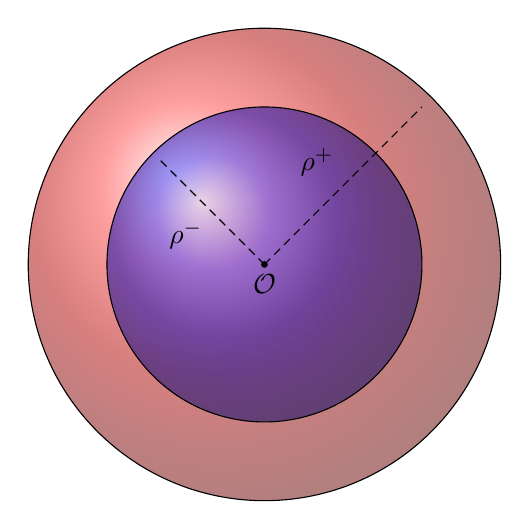
\begin{tikzpicture}
      \coordinate (O) at (0,0);
      
      % outer ball background color
      \shade[ball color = red, opacity = 0.5] (0,0) circle [radius = 3cm];
    
      %outer ball ball
      \draw (O) circle [radius=3cm];
    
      % inner ball background color
      \shade[ball color = blue, opacity = 0.5] (0,0) circle [radius = 2cm];
    
      % inner ball
      \draw (O) circle [radius=2cm];
      % label of ball center point
      \filldraw (O) circle (1pt) node[below] {$\mathcal{O}$};
    
      % radius for inner ball
      \draw[densely dashed] (O) to [edge label = $\rho^-$] (-1.33,1.33);
      % radius for outer ball
      \draw[densely dashed] (O) to [edge label = $\rho^+$] (2,2);
      
    
    \end{tikzpicture}
      \caption{Concentric hyper-spheres of radii $\rho^-,\rho^+$. Channel norms are restricted to this range in order to project vectors onto the surface of a hyper-sphere of constant radius. In order to pessimistically lower bound orthogonality probabilities, the larger radius of $\rho^+$ is chosen. The probability channel norms will fall into this range can be described in terms of channel fading statistics.}
    \label{fig:concentric_sphere}
\end{figure}
  
The CDF of the channel norm will be denoted by $F_{\Vert\underline{hi}\Vert^2}(m,\rho)$, where $\rho$ are realizations of the random variable formed by the channel norm. Each term in the $N$-length vector, $\underline{h}_i$ is represented by two iid normal random variables: one for the real part and one for the imaginary part. When forming the L2 norm of the $N$-length vector, each multiplication forms a sum of length four where each of the arguments of the sum are a product of two random variables. Namely, the sum takes the form real$\cdot$real + real$\cdot$imaginary + imaginary$\cdot$real + imaginary$\cdot$imaginary. Thus, the CDF expression becomes:
\begin{equation}\label{eq:ch_sq_cdf_chan}
    \begin{aligned}
        F_{\Vert\underline{hi}\Vert^2}(\rho;m)& = \Gamma_n(2m,m\rho)\\
        &= Pr[\Vert\underline{h}_i\Vert^2 \leq \rho]
    \end{aligned}
\end{equation}
where $\Gamma_n(\cdot)$ is the incomplete normalized gamma function.

The probability that $\Vert\underline{h}_i\Vert^2$ lands in the shell between radii $\rho^+,\ \rho^-$,  is given by the subtraction of the respective CDF expressions:
\begin{equation}\label{eq:p_s}
    \begin{aligned}
        p_s = \Gamma_n(2N,N\rho^-) - \Gamma_n(2N,N\rho^+)
    \end{aligned}
\end{equation}

The issue of resolving the projection of channel vectors onto the surface of a sphere is still not entirely resolved: we have only described the probability the vectors will exist in a shell defined by upper and lower bounding radii. In order to pessimistically bound orthogonality analysis in the upcoming discussion, it is assumed that all the channel norms that exist in the shell are equal to $\rho^+$. In this way, we have a trade-off between probability of channel norms existence and accuracy of orthogonality analysis: as ${(\rho^+-\rho^-)\rightarrow 0},\ p_s\rightarrow 0$; however, as  $(\rho^+-\rho^-)$ grows, so does the inaccuracy in orthogonality analysis.



    \section{Semi-orthogonality of points on spherical surface}
        Orthogonality between pairs of vectors can be interpreted geometrically on the spherical surface in terms of spherical caps. A spherical cap is formed on the surface of the hyper-sphere of radius $\rho^+$ by by first extending the channel vector $\underline{h_i}$ onto the spherical surface as described in Section \ref{sec:chan_norm}. Then a cone, with its apex at $\mathcal{O}$, with half angle $\theta$, centered along the axis of $\underline{h_i}$ is intersected with the spherical surface. This intersection defines a spherical cap. $\mathcal{C}_i$. This process is illustrated in Fig. \ref{fig:spherical_cap}. 

considering a spherical surface with two vectors touching the surface of the sphere at arbitrary points on the sphere. A measure of orthogonality between these vectors can easily be calculated by forming the inner product between these vectors. Alternatively we could form a cone for each vector. The apex of each cone is the origin of the sphere, $\mathcal{O}$. The half angle of each cone is given by $\theta$.

\begin{figure}
\centering
    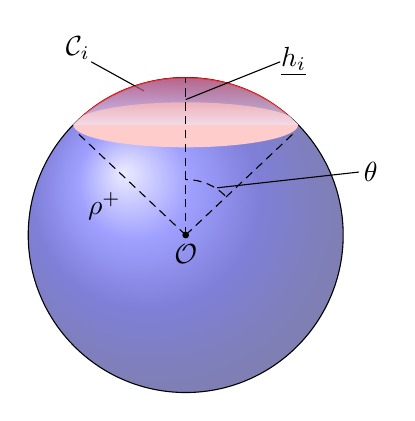
\begin{tikzpicture}%[font = \sansmath]
        %define origin, 1-height of cone, radius
        \coordinate (O) at (0,0);
        \def\r{2}
        \def\H{.6}
        
        \begin{scope}
        % ball background color
        \shade[ball color = blue, opacity = 0.5] (0,0) circle [radius = \r];
        
        % cone
        \begin{scope}
            \def\rx{0.71}% horizontal radius of the ellipse
            \def\ry{0.15}% vertical radius of the ellipse
            \def\z{0.725}% distance from center of ellipse to origin
        
            \path [name path = ellipse]    (0,\z) ellipse ({\rx} and {\ry});
            \path [name path = horizontal] (-\rx,\z-\ry*\ry/\z)
                                        -- (\rx,\z-\ry*\ry/\z);
            \path [name intersections = {of = ellipse and horizontal}];
        
            %% radius to base of cone in ball
            %\draw[fill = gray!50, gray!50] (intersection-1) -- (0,0)
            %  -- (intersection-2) -- cycle;
            %% base of cone in ball
            %\draw[fill = gray!30, densely dashed] (0,\z) ellipse ({\rx} and %{\ry});
        \end{scope}
        
        % label of cone
        %\draw (0.25,0.4) -- (0.9,0.1) node at (1.05,0.0) {$q$};
        
        % ball
        \draw (O) circle [radius=2cm];
        
        % label of ball center point
        \filldraw (O) circle (1pt) node[below] {$\mathcal{O}$};
        
        % radius
        \draw[densely dashed] (O) to [edge label = $\rho^+$] (-1.4,1.32);
        \draw[densely dashed] (O) -- (1.4,1.32);
        %label colatitude angle
        \draw[densely dashed] (0.5,0.5) arc [start angle = 45, end angle = 90, x radius = 7mm, y radius = 7mm];
        \draw (2.2, 0.8) -- (0.4, 0.6) node at (2.35,0.8) {$\theta$};
        
        % cut of ball surface
        \draw[red] (-1.35,1.47) arc [start angle = 140, end angle = 40, x radius = 17.6mm, y radius = 14.75mm];
        %\draw[red, densely dashed] (-1.36,1.46) arc [start angle = 170, end angle = 10,
        x radius = 13.8mm, y radius = 3.6mm];
        %\draw[red] (-1.29,1.52) arc [start angle=-200, end angle = 20,
        x radius = 13.75mm, y radius = 3.15mm];
        
        % label of cut of ball surface
        \draw (-1.2,2.2) -- (-0.53,1.83) node at (-1.37,2.37) {$\mathcal{C}_i$};
        
        %shade the spherical cap
        \begin{scope}
            %clip the shading outside the ball
            \clip ({\r*cos(-90)},{\r*sin(-90)}) arc [start angle=-90,end angle=270,radius=\r];
            %draw the disk    
            \fill[red!20] (0,{\r-\H}) circle [x radius={sqrt(\r^2-(\r-\H)^2)}, y radius={0.2*sqrt(\r^2-(\r-\H)^2)}];
            %shade the disk
            \shade[top color=red!70!gray,bottom color=red!10!blue!10!,opacity=0.6]  ({\r},{1.1*\r}) rectangle ++({-2*\r},{-0.1*\r-\H});
        \end{scope}
    
        %draw channel vector
        \draw[densely dashed] (O) -- (0,2);
        %label channel vector
        \draw (1.2,2.2) -- (0,1.72) node at (1.37,2.2) {$\underline{h_i}$};
        \end{scope}
    \end{tikzpicture}
    
    \caption{Surface of hyper-sphere in 2$N$ dimensions. A spherical cap, $\mathcal{C}_i$ is shown (shaded in red). $\mathcal{C}_i$ is formed by projecting the channel vector, $\underline{h_i}$, onto the spherical surface. A colatitude angle of $\theta$ and radius of $\rho^+$ are assumed in forming $\mathcal{C}_i$. Alternatively, $\mathcal{C}_i$ can also be interpreted as the cap formed by intersecting a cone of half-angle $\theta$ with the spherical surface.}
    \label{fig:spherical_cap}
\end{figure}
    \section{Sum of dependent random indicator variables}
    \section{Semi-orthogonal group existence probability}

    \newpage

	%\section{Appendices}
	    %\subsection{Notes on Gamma-distributed variables}
	    %    \input{app/gamma_dist.tex}
    \newpage	
 	\begingroup
 		\renewcommand{\section}[2]{}%
 		\bibliographystyle{IEEEtran}
 		\bibliography{references}
 	\endgroup
\end{document}
